\documentclass{article} % A4 paper and 11pt font size
\setcounter{secnumdepth}{0}

\usepackage{amssymb, amsmath, amsfonts}
\usepackage{moreverb}
\usepackage{graphicx}
\usepackage{enumerate}
\usepackage{graphics}
\usepackage[margin=1in]{geometry}
\usepackage{color}
\usepackage{tocloft}
\renewcommand{\cftsecleader}{\cftdotfill{\cftdotsep}}
\usepackage{array}
\usepackage{float}
\usepackage{csquotes}
\usepackage{placeins}
\usepackage{verbatim}
\usepackage{hyperref}
\usepackage{textcomp}
\usepackage[makeroom]{cancel}
\usepackage{bbold}
\usepackage{scrextend}
\usepackage{alltt}
\usepackage{listings}
\usepackage{physics}
\usepackage{mathtools}
\usepackage[normalem]{ulem}
\usepackage{amsthm}
\usepackage{tikz}
\usetikzlibrary{positioning}
\usetikzlibrary{arrows}
\usepackage{pgfplots}
\usepackage{bigints}
\allowdisplaybreaks
\pgfplotsset{compat=1.12}

\theoremstyle{plain}
\newtheorem*{theorem*}{Theorem}
\newtheorem{theorem}{Theorem}
\newtheorem*{lemma*}{Lemma}
\newtheorem{lemma}{Lemma}

\definecolor{verbgray}{gray}{0.9}
% \definecolor{dkgreen}{green}{0.9}

\lstnewenvironment{code}{%
  \lstset{
  language=R,
  backgroundcolor=\color{verbgray},
  keywordstyle=\color{blue},      % keyword style
  commentstyle=\color{magenta},   % comment style
  stringstyle=\color{olive},      % string literal styleframe=single,
  numberstyle=\color{black},      % string literal styleframe=single,
  framerule=0pt,
  numbers=left,
  stepnumber=1,
  firstnumber=1,
  showspaces=false,
  basicstyle=\ttfamily}}{}

\lstnewenvironment{console_output}{%
  \lstset{
  framerule=0pt,
  numbers=left,
  stepnumber=1,
  showspaces=false,
  firstnumber=1,
  basicstyle=\ttfamily}}{}


\makeatletter
\newcommand{\BIGG}{\bBigg@{3}}
\newcommand{\vast}{\bBigg@{4}}
\newcommand{\Vast}{\bBigg@{5}}
\makeatother

\newenvironment{definition}[1][Definition]{\begin{trivlist}
\item[\hskip \labelsep {\bfseries #1}]}{\end{trivlist}}

\newcommand{\dy}{\partial_y}
\newcommand{\dyy}{\partial_{yy}}
\newcommand{\dxx}{\partial_{xx}}
\newcommand{\dxy}{\partial_{xy}}
\newcommand{\dyyy}{\partial_{yyy}}
\newcommand{\dxxx}{\partial_{xxx}}
\newcommand{\dx}{\partial_x}
\newcommand{\E}{\varepsilon}
\def\Rl{\mathbb{R}}
\def\Cx{\mathbb{C}}

\newcommand{\Ei}{\text{Ei}}

\usepackage[T1]{fontenc} % Use 8-bit encoding that has 256 glyphs
\usepackage{fourier} % Use the Adobe Utopia font for the document - comment this line to return to the LaTeX default
\usepackage[english]{babel} % English language/hyphenation

\usepackage{sectsty} % Allows customizing section commands
\allsectionsfont{\centering \normalfont\scshape} % Make all sections centered, the default font and small caps

\usepackage{fancyhdr} % Custom headers and footers
\pagestyle{fancy} % Makes all pages in the document conform to the custom headers and footers
\fancyhead[L]{\bf Sam Fleischer}
\fancyhead[C]{\bf UC Davis \\ Principles of Population Biology (PBG200A)} % No page header - if you want one, create it in the same way as the footers below
\fancyhead[R]{\bf Fall 2016}

\fancyfoot[L]{\bf } % Empty left footer
\fancyfoot[C]{\bf \thepage} % Empty center footer
\fancyfoot[R]{\bf } % Page numbering for right footer
\renewcommand{\headrulewidth}{0pt} % Remove header underlines
\renewcommand{\footrulewidth}{0pt} % Remove footer underlines
\setlength{\headheight}{25pt} % Customize the height of the header

\newcommand{\VEC}[2]{\left\langle #1, #2 \right\rangle}
\newcommand{\expec}[1]{\mathbb{E}\qty[#1]}
\newcommand{\prob}[1]{\mathbb{P}\qty[#1]}
\newcommand{\vari}[1]{\text{var}\qty[#1]}
\newcommand{\ran}{\text{\rm ran }}
\newcommand{\Hilb}{\mathcal{H}}
\newcommand{\lap}{\Delta}

\newcommand{\littleo}[1]{\text{\scriptsize$\mathcal{O}$}\qty(#1)}

\DeclareMathOperator*{\esssup}{\text{ess~sup}}

\newcommand{\problem}[2]{
\vspace{.375cm}
\boxed{\begin{minipage}{\textwidth}
    \section{\bf #1}
    #2
\end{minipage}}
}

\numberwithin{equation}{section} % Number equations within sections (i.e. 1.1, 1.2, 2.1, 2.2 instead of 1, 2, 3, 4)
\numberwithin{figure}{section} % Number figures within sections (i.e. 1.1, 1.2, 2.1, 2.2 instead of 1, 2, 3, 4)
\numberwithin{table}{section} % Number tables within sections (i.e. 1.1, 1.2, 2.1, 2.2 instead of 1, 2, 3, 4)

\setlength\parindent{0pt} % Removes all indentation from paragraphs - comment this line for an assignment with lots of text

\newcommand{\horrule}[1]{\rule{\linewidth}{#1}} % Create horizontal rule command with 1 argument of height

\title{ 
\normalfont \normalsize 
\textsc{UC Davis, Principles of Population Biology (PBG 200A), Fall 2016} \\ [25pt] % Your university, school and/or department name(s)
\horrule{2pt} \\[0.4cm] % Thin top horizontal rule
\Huge Homework \#2 \\ % The assignment title
\horrule{2pt} \\[0.5cm] % Thick bottom horizontal rule
}

\author{\huge Sam Fleischer} % Your name

\date{October 19, 2016} % Today's date or a custom date

\begin{document}\thispagestyle{empty}

\maketitle % Print the title

\makeatletter
\@starttoc{toc}
\makeatother

\pagebreak

%%%%%%%%%%%%%%%%%%%%%%%%%%%%%%%%%%%%%%
\problem{Problem 1}{Consider a population of annual plants whose seed bank has abundance $N(t)$ in year $t$.  The probability that a seed germinates in a given year is $G$.  The percentage of non-germinating seeds that survive to the next year is $70\%$.  On a good year, a germinating seed contributes (on average) $6$ seeds to the next years seed bank.  On a bad year, one in eight germinating seeds contribute (on average) one seed to the next years seed bank.  Each year the probability of a good year is $0.5$ independent of other years.
\begin{enumerate}[\ \ (a)]
    \item If all seeds germinate in their first year (i.e.~$G=1$) and the initial density of seeds is $100$, find their expected density ten years from now.  Will this population of seeds persist in the long-term?  Justify your answers.
    \item Write down an expression, call it $r(G)$, for the expected value of the logarithmic fitness of the population as a function of $G$.  Use \texttt{R} to plot this function.  For what values of $G$, if any, does the population persist?  What is the ``optimal value'' for $G$?  What rate does the population grow for this optimal germination strategy?
    \item Discuss what types of changes in the environment (e.g.~probability of a good year, survivorship of seeds, etc.) would result in a lower optimal value of $G$.  Also discuss how these environmental changes would effect the growth rate of the population i.e.~effect $r(G)$.
\end{enumerate}}

\begin{enumerate}[\ \ (a)]
    \item
        The following model arises:
        \begin{align}
            N_{t+1} = N_t\qty(GY_{t+1} + (1 - G)S)
        \end{align}
        where $G$ is the probability a seed germinates and $Y$ is a random variable describing seed yield for germinating plants in a particular year.  $S = 0.7$ is the probability a seed in the seed bank survives.  The parameters given are $Y_{t+1} = \left\{6,\frac{1}{8}\right\}$, each with probability $0.5$, with no correlation.  If $G = 1$ and $N_0 = 100$, the model is 
        \begin{align}
            N_{t+1} = N_tY_{t+1} \qquad N_0 = 100
        \end{align}
        and thus
        \begin{align}
            N_{10} = N_0\prod_{t=1}^{10}Y_{t} \implies \expec{N_{10}} = 100\expec{\prod_{t=1}^{10}Y_t} \implies \log(\expec{N_{10}}) = \log(100) + \sum_{t=1}^{10}\expec{\log(Y_t)}
        \end{align}
        but $r \coloneqq \expec{\log(Y_t)} \approx -0.144$, and so $\log(\expec{N_{10}}) \approx 3.167$, which implies $\expec{N_{10}} = 23.73$.  The population of seeds will not persist in the long-term since $r < 0$.  The bad years are worse than the good years are good.
    \item
        
\end{enumerate}












%%%%%%%%%%%%%%%%%%%%%%%%%%%%%%%%%%%%%%
\problem{Problem 2}{Consider two populations, $A$ and $B$, that can be modeled by $$N(t+1) = R(t)N(t)$$ with $N_0 = 500$.  For population $A$, $R(t)$ has been observed to take on the following values $$\{1.1, 0.9, 1.2, 0.8\}.$$  For population $B$, $R(t)$ has been observed to take on the following values $$\{2.0, 0.4, 3.0, 0.5\}.$$
\begin{enumerate}[\ \ (a)]
    \item Compute the expected values and variances for $\ln R(t)$.  Discuss the long-term fate of each of these populations.
    \item For each population, estimate the probability that $N_{25} \leq 100$.  Discuss these predictions.
    \item How do your predictions for (b) change if you were told that the correlation between $\ln R(t)$ and $\ln R(t+1)$ equals $\rho^t$ where $\rho$ equals $0.5$ for population $A$ but $-0.5$ for population $B$?  Discuss.
\end{enumerate}}

\begin{enumerate}[\ \ (a)]
    \item
        \begin{enumerate}[Pop.~A:\ ]
            \item
                $\ln R(t)$ takes the values $\{\ln1.1, \ln0.9, \ln1.2, \ln0.8\}$ with equal probabilities, and thus $\mu_A = \expec{\ln R(t)} = -0.013$ with $\sigma_A^2 = \vari{\ln R(t)} = 0.256$.
            \item
                $\ln R(t)$ takes the values $\{\ln2,\ln0.4,\ln3,\ln0.5\}$ with equal probabilities, and thus $\mu_B = \expec{\ln R(t)} = 0.456$ with $\sigma_B^2 = \vari{\ln R(t)} = 0.750$.
        \end{enumerate}
    \item
        \begin{enumerate}[Pop.~A:\ ]
            \item
                For $N_0 = 500$,
                \begin{align}
                    \prob{N_{25}\leq 100} = \prob{\frac{\log \dfrac{N_{25}}{500} - 25\mu_A}{5\sigma_A} \leq \frac{\log\dfrac{100}{500} - 25\mu_A}{5\sigma_A}}
                \end{align}
                This is easy to calculate since $X = \dfrac{\log \frac{N_{25}}{500} - 25\mu_A}{5\sigma_A}$ is standard normal so $z_A = \dfrac{\log\frac{100}{500} - 25\mu_A}{5\sigma_A} \approx -1.317$ is a $z$-score.  This corresponds to a $9.4\%$ probability the population is below $100$ at the $25$th timestep.
            \item
                For $N_0 = 500$,
                \begin{align}
                    \prob{N_{25}\leq 100} = \prob{\frac{\log \dfrac{N_{25}}{500} - 25\mu_B}{5\sigma_B} \leq \frac{\log\dfrac{100}{500} - 25\mu_B}{5\sigma_B}}
                \end{align}
                This is easy to calculate since $X = \dfrac{\log \frac{N_{25}}{500} - 25\mu_B}{5\sigma_B}$ is standard normal so $z_B = \dfrac{\log\frac{100}{500} - 25\mu_A}{5\sigma_A} \approx -0.823$ is a $z$-score.  This corresponds to a $20.1\%$ probability the population is below $100$ at the $25$th timestep.
        \end{enumerate}
        This probabilities are shown in simulations.  Note that the upward trend for population B is initially not enough to overcome the large variance in growth rate, at least initially.  The next graph is a simulation for $2000$ timesteps.  Note that the positive trend for population B eventually overcomes the large variance.  In general, population A will go extinct as $t \rightarrow \infty$ with probability $1$, and population B will grow to infinity as $t \rightarrow \infty$ with probability $1$.
        \begin{figure}[ht!]
            \centering
            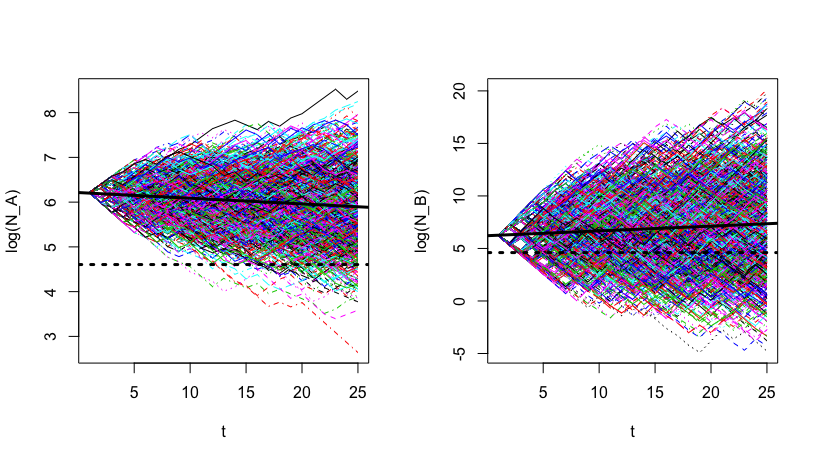
\includegraphics[scale=0.4]{figure_2b1.png}
            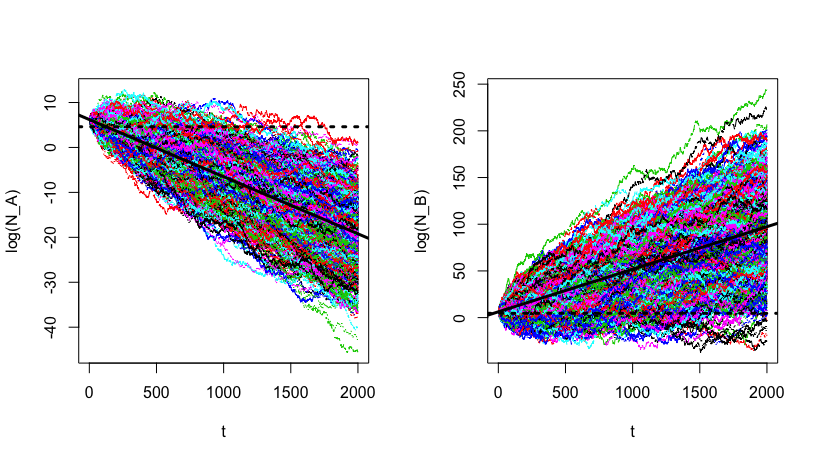
\includegraphics[scale=0.4]{figure_2b2.png}\\
            Left: Population A.  Right: Population B.  Solid line shows trend.  Dotted line shows $N=100$ threshold.
        \end{figure}
        \FloatBarrier
    \item
        {\color{red} Something about correlations}
\end{enumerate}













%%%%%%%%%%%%%%%%%%%%%%%%%%%%%%%%%%%%%%
\problem{Problem 3}{In a 1995 Science article entitled ``Population Dynamics of Exploited Fish Stocks at Low Population Levels'' by R.~A.~Myers and colleagues, parameterized a model of the following form $$N(t+1) = \frac{R(t)N(t)^b}{1 + a N(t)^b}$$ for various fish species.  In this model, $a > 0$ is the intraspecific competition coefficient, $R(t)$ is a measure of intrinsic fitness, and $b$ is called the ``dispensation'' parameter.  When $b > 1$,  the model exhibits an Allee effect, i.e.~positive density dependence at low densities.  In this problem, you will investigate the combined effects of environmental stochasticity and Allee effects on population persistence.  Assume that $\ln R(t)$ is normally distributed in time with mean $\mu = -2.5$ and standard deviation $\sigma$.  More specificially, to allow for temporal correlations $\ln R(t)$ defined as follows
\begin{align*}
    \ln[R(t+1)]\ &=\ \mu + \sigma \eta_t \\
    \eta_{t+1}\ &=\ \rho \eta_t + \sqrt{1 - \rho^2}Z_t
\end{align*}
where $Z_1,Z_2,\dots$ are independent and identically distributed standard normals.  $\rho$ measures the correlation between $R(t)$ and $R(t+1)$.  For these explorations, assume that $a = 0.001$, $b = 2$, and $\mu = -2.5$.
\begin{enumerate}[\ \ (a)]
    \item Assuming that $\sigma = 0$ (i.e.~$R = e^{-2.5}$ for all time), find and plot the per-capita growth rate function $R(N)$.  Use your plot to estimate (to the nearest integer) the two positive equilibria of the model.  Call the lower one $N_*$ and the upper one $N^*$.
    \item Simulate the population dynamics with initial abundance $N^*$ for $200$ time steps with different values of $\sigma$ and $\rho$.  Discuss how these two parameters influence the population dynamics.
    \item To understand how $\sigma$ influences population persistence, consider $\rho = 0$ and $\sigma = 0.1, 0.2, 0.3, 0.4, 0.5$.  For each $\sigma$ value, have \texttt{R} simulate the dynamics (starting at $N^*$) for 200 time steps for $1,000$ reps (to determine the fraction of reps for which the population persisted $200$ time steps).  Discuss how the probability of extinction in two centuries depends on the level of noise.  Discuss the conservation implications.
    \item To understand how $\rho$ influences population persistence, repeat (c) with $\rho = -0.5$ and $\rho = 0.5$.  Discuss what you observe and the conservation implications.
\end{enumerate}}

\begin{enumerate}[\ \ (a)]
    \item
        Assuming $\sigma = 0$ and thus $R_t = e^{-2.5}$, and since $a = 0.001$ and $b = 2$, we have
        \begin{align}
            N_{t+1} = \frac{e^{-2.5} N_t^2}{1 + 0.001N_t^2}
        \end{align}
        To find equilibria, set $N = N_{t+1} = N_t$ and solve for $N$.
        \begin{align}
            N &= \frac{e^{-2.5}N^2}{1 + 0.001N^2} \\
            \implies N - e^{-2.5}N^2 + 0.001N^3 &= 0 \\
            \implies N\qty(1 - e^{-2.5}N + 0.001N^2) &= 0 \\
            \implies N &\approx 0,\ 14.88,\ 67.21
        \end{align}
        So $N_* \approx 14.88$ and $N^* \approx 67.21$.  Graphically, we plot $N_{t+1}$ vs.~$N_t$ and see where the plot intersects with $N_{t+1} = N_{t}$:
        \begin{figure}[ht!]
            \centering
            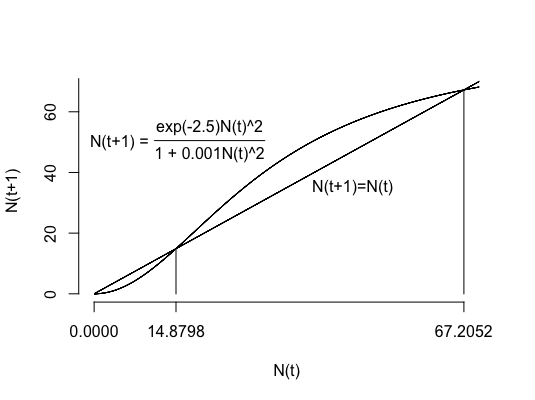
\includegraphics[scale=0.5]{figure_3a.png}
        \end{figure}
        \FloatBarrier
    \item
        Based on simulations, if $R_{t+1}$ is strongly negatively correlated to $R_t$ ($\rho$ close to $-1$), then high variability in environmental conditions (high $\sigma$) do not affect persistence.  However if $R_{t+1}$ is strongly positively correlated with $R_t$ ($\rho$ close to $1$), then high variability in environmental conditions is devastating for persistence. T
        \begin{figure}[ht!]
            \centering
            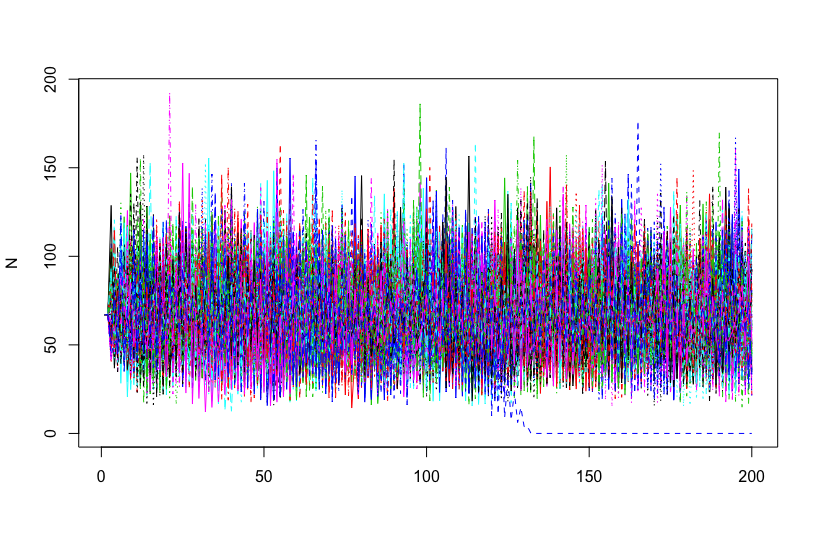
\includegraphics[scale=0.4]{figure_3b1.png}\\
            Strong negative correlation in environmental conditions, high variability
        \end{figure}
        \begin{figure}[ht!]
            \centering
            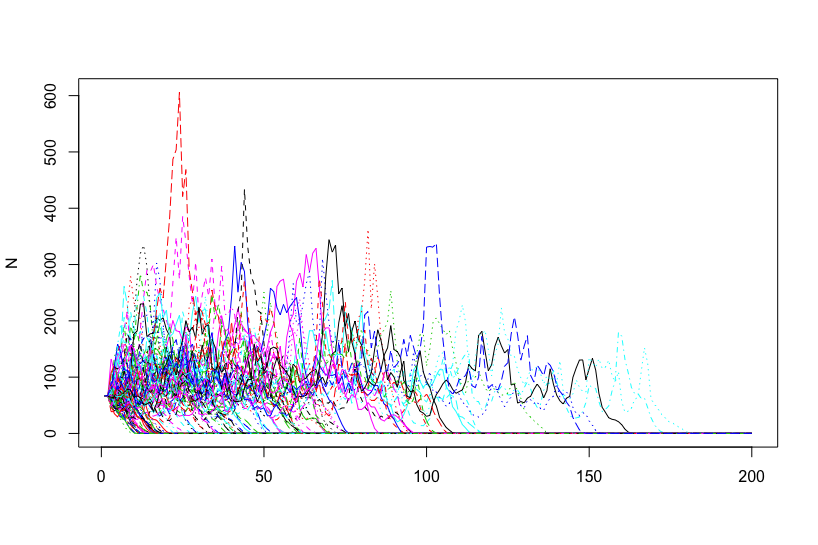
\includegraphics[scale=0.4]{figure_3b2.png}\\
            Strong positive correlation in environmental conditions, high variability
        \end{figure}
        \FloatBarrier
    \item
        Here are the results for $\rho = 0$:
        \begin{align}
            \begin{array}{||l|l||}\hline\hline
                \sigma & \text{fraction extinct} \\\hline
                0.1 & 0/1000 \\\hline
                0.2 & 0/1000 \\\hline
                0.3 & 87/1000 \\\hline
                0.4 & 553/1000 \\\hline
                0.5 & 931/1000 \\\hline\hline
            \end{array}
        \end{align}
        Clearly the probability of extinction is an increasing function with the level of noise in environmental conditions.  This means increased variability in environmental conditions is detrimental to persistence, so if we expect variability to increse as climate change becomes more extreme, we must take extra measures to preserve natural populations.
    \item
        \begin{align}
            \begin{array}{cc}
                \rho = -0.5 & \rho = 0.5 \\
                \begin{array}{||l|l||}\hline\hline
                    \sigma & \text{fraction extinct} \\\hline
                    0.1 & 0/1000 \\\hline
                    0.2 & 0/1000 \\\hline
                    0.3 & 0/1000 \\\hline
                    0.4 & 9/1000 \\\hline
                    0.5 & 169/1000 \\\hline\hline
                \end{array} & \begin{array}{||l|l||}\hline\hline
                    \sigma & \text{fraction extinct} \\\hline
                    0.1 & 0/1000 \\\hline
                    0.2 & 73/1000 \\\hline
                    0.3 & 701/1000 \\\hline
                    0.4 & 958/1000 \\\hline
                    0.5 & 999/1000 \\\hline\hline
                \end{array}
            \end{array}
        \end{align}
        These results agree with my analysis in part (b).  Negative correlation ensures bad years are followed by good years, which helps alleviate their devastating affects.  On the other hand, positive correlation ensures bad years are followed by more bad years, which may push species under the critical threshold $N_*$, making it virtually impossible to climb back to persistence.
\end{enumerate}












%%%%%%%%%%%%%%%%%%%%%%%%%%%%%%%%%%%%%%
\problem{Problem 5}{(Effects of correlations between vital rates on growth)
\begin{enumerate}[\ \ (a)]
    \item Consider three annual plant populations in which $50\%$ of the seeds germinate every year.  Good years and bad years occur with equal likelihood.  In good years for the seeds, $90\%$ survive, otherwise only $50\%$ survive.  In good years for the plants, $4$ seeds are produced that enter the seed bank, otherwise only $1$ in $5$ plants produces a seed that enters the seed bank.  The populations differ in the following way:
    \begin{addmargin}[1em]{2em}
        \textbf{Population A:} Good (respectively bad) years for the seeds are also good (respectively bad) years for the plants.  In other words, environmental conditions corresponding to good years for the plants are perfectly correlated with environmental conditions corresponding to good years for the seeds.

        \textbf{Population B:} Good years for the seeds are bad years for the plants, and vice versa.  In other words, environmental conditions corresponding to good years for the plants are perfectly negatively correlated with good years with the seeds.

        \textbf{Population C:} Environmental conditinos corresponding to good years for the plants versus good years for the seeds are independent of one another.
    \end{addmargin}
    Compute the geometric growth rate of each of these populations and discuss your findings.
    \item More generally, consider an iteroparous population whose dynamics are given by $N_{t+1} = (S_t + F_t)N_t$ where $S_t$ is the fraction of individuals that survive to the next time step and $F_t$ is the mean number of offspring per individual at time $t$.  Use the small variance approximation of the stochastic growth rate to demonstrate the effects of correlations between $S_t$ and $F_t$ on the long-term population growth rate.
\end{enumerate}}

\begin{enumerate}[\ \ (a)]
    \item
        In class we discussed the following bet-hedging model for annual plants with seed banks
        \begin{align*}
            N_{t+1} = N_t\qty[gY_{t+1} + (1-g)S]
        \end{align*}
        where $N$ is the number of seeds underground, $g$ is the probability of germination, germination produces yield $Y_{t+1}$ (which is a random variable based on good or bad years for the plants), and $S$ is the probability a seed in the seed bank survives.  For this problem, however, we must consider $S = S_{t+1}$ to be a random variable based on good or bad years for the seeds.
        \begin{align*}
            N_{t+1} = N_t\underbrace{\qty[gY_{t+1} + (1-g)S_{t+1}]}_{=R_{t+1}}
        \end{align*}
        This problem specifies $g = .5$, $Y_{t+1}$ is a discrete random variable which takes the values $4$ or $0.2$ with $50\%$ probabilities.  $S_{t+1}$ takes the values $0.9$ or $0.5$ with $50\%$ probabilities.  Good years for the plants and seeds correspond to $Y_{t+1} = 4$ and $S_{t+1} = 0.9$ and bad years correspond to $Y_{t+1} = 0.2$ and $S_{t+1} = 0.5$.  This problem explores the effects of correlation of these random variables on the long-term dynamics of the model.
        \begin{enumerate}[Pop.~A:\ ]
            \item
                Assuming $Y$ and $S$ are perfectly positively correlated, then the random variable $R = gY + (1-g)S$ takes the values $2.45$ or $0.35$ with $50\%$ probabilities.  Thus,
                \begin{align*}
                    r = \expec{\ln(R)} \approx -0.07686 < 0
                \end{align*}
                which shows this population will asymptotically go extinct.
            \item
                Assuming $Y$ and $S$ are perfectly negatively correlated, then the random variable $R = gY + (1-g)S$ takes the values $2.25$ or $0.55$ with $50\%$ probabilities.  Thus,
                \begin{align*}
                    r = \expec{\ln(R)} \approx 0.1065 > 0
                \end{align*}
                which shows this population will grow exponentially.
            \item
                Assuming $Y$ and $S$ are uncorrelated, then the random variable $R = gY + (1-g)S$ takes the values $2.45$, $2.25$, $0.55$, or $0.35$ with $25\%$ probabilities.  Thus,
                \begin{align*}
                    r = \expec{\ln(R)} \approx 0.0148 > 0
                \end{align*}
                which shows this population will grow exponentially, but at a much slower rate than population B.
        \end{enumerate}
        The intuition here is that it is the magnitude of bad years which makes the biggest difference on long-term growth (because of the log transformation).  In population A, even though good years are exceptionally good, the bad years are exceptionally bad, which drives the population to extinction.  In population B, the good years are less good, but the bad years are less bad, which enables the population to survive.
    \item
        Consider an iteroparous population with dynamics
        \begin{align*}
            N_{t+1} = (S_t + F_t)N_t
        \end{align*}
        where $S_t$ is survivability and $F_t$ is fecundity.  Defining $R_t \coloneqq S_t + F_t$, and assuming $\vari{R}$ is small, then $R = \bar{R} + \sigma X$ where $\bar{R}$ is $\expec{R}$, $\sigma$ is small, and $X$ is a normal distribution with mean $0$ and variance $1$.
        \begin{align*}
            r = \expec{\log[R_1]} = \expec{\log(\bar{R} + \sigma X)} = \log(\bar{R}) + \expec{\log(1 + \frac{\sigma}{\bar{R}}X)}
        \end{align*}
        However, $\log(1 + x) = x - \frac{1}{2}x^2 + \order{x^3}$, so for small $x$ we can use $\log(1 + x) \approx x - \frac{1}{2}x^2$, so
        \begin{align*}
            r \approx \log(\bar{R}) + \expec{\frac{\sigma}{\bar{R}}X - \frac{1}{2}\qty(\frac{\sigma}{\bar{R}}X)^2} = \log(\bar{R}) - \frac{1}{2}\qty(\frac{\sigma}{\bar{R}})^2
        \end{align*}
        {\color{red} something about correlations..}
\end{enumerate}












%%%%%%%%%%%%%%%%%%%%%%%%%%%%%%%%%%%%%%
\problem{Problem 6}{For the checkerspot model, compute $r_0$ for the pre-1971 rainfall and post-1970 rainfall data.  Discuss whether these numbers provide insights consistent with running the full nonlinear model.}














\end{document}
